\documentclass[11pt,a4paper]{report}
\usepackage{graphicx}
\usepackage{float}
\textwidth=450pt
\oddsidemargin=0pt
\begin{document}

\title{Title}

\section*{Brain Challenge}
This project aim to analyze the relationship between a bunch of features computed on several NRM images of the brain of different patients and the age of those patients. The final purpose of this analysis is to attempt to detect those images' features that are better able to predict the patient's age and try to extract the biological meaning from this information. Some simple regression methods performed well on the entire dataset and received a $R^{2} = 0.792$, but the aim was to find a restricted set of features with a not so lower score. I've found out that a restricted set of 50 features was able to predict the age of the sample with a $R^{2}$ equal to ????.



\subsection*{Material and Methods}
Where do the images come from???
The raw images database had already been pre-processed when it was given to me. Therefore my work started with a dataframe with about 1000 features collected on almost 2000 samples (\texttt{n\_features} = 954 and \texttt{n\_samples} = 2364). I've written all the necessaries scripts using Python and more precisely I've exploited a lot of methods form the package \texttt{scikitlearn}.

\subsection*{Dimensionality Reduction}
The reduction in the number of features is one of the key point of this analysis. I wanted to conserve the meaning of each features in the reduced space so I avoided the use of any dimensionality reduction method that worked with a combination of features as PCA or ???. What I've looked for was a method to score the importance of any feature in the prediction of the age of the subject. Hence I used different combinations of scaler method, to standardize the data, and penalized linear model like ridge, Lasso and the elastic net. The coefficients of theese regressions have been used as scores in the determination of which were the most predictive features.

More precisely, I used three different method to standardize the data: the \texttt{MinMaxScaler}, the \texttt{StandardScaler} and the \texttt{RobustScaler}. The \texttt{MinMaxScaler} scales the each feature individually to the range $\lbrack 0,1 \rbrack$, and it's the one that received the best scores among the three. The \texttt{StandardScaler} modify each single column simply setting the mean to 0 and the standard deviation to 1. The \texttt{RobustScaler} instead, manage every feature giving less importance to outliers.

Those scaling methods were combined with three penalized regression methods: the \texttt{LassoCV}, the \texttt{RidgeCV}, and the \texttt{ElasticNetCV}.All these three supervised methods are linear in the coefficients. What you obtain after such a regression is the array of values that express the linear combination of features that better predict the age of the samples. Every one of these methods find the best hyper-parameters for the regression and perform automatically a cross validation on their results.  The Lasso regression exerts a penalization on the L1-norm of the coefficients vector, the ridge regression instead is based on the L2-norm of the vector, while the elastic net method performs a sort of mixture of the two methods.

The total number of combinations among these elements is 9. So I processed the data with each one of them and obtained nine arrays of coefficients. Then I was able to sort the absolute values of those coefficients in order to find the most important ones for every combination. The idea was to select a certain number of the most influential features and use them to perform further analysis. These results are shown in Figure \ref{fig:NineCoefPlot}. The 9 sets of values reported in \ref{fig:NineCoefPlot} were used to find those values to use as thresholds in selecting the most important features.

\begin{figure}[ht!]
  \begin{center}
  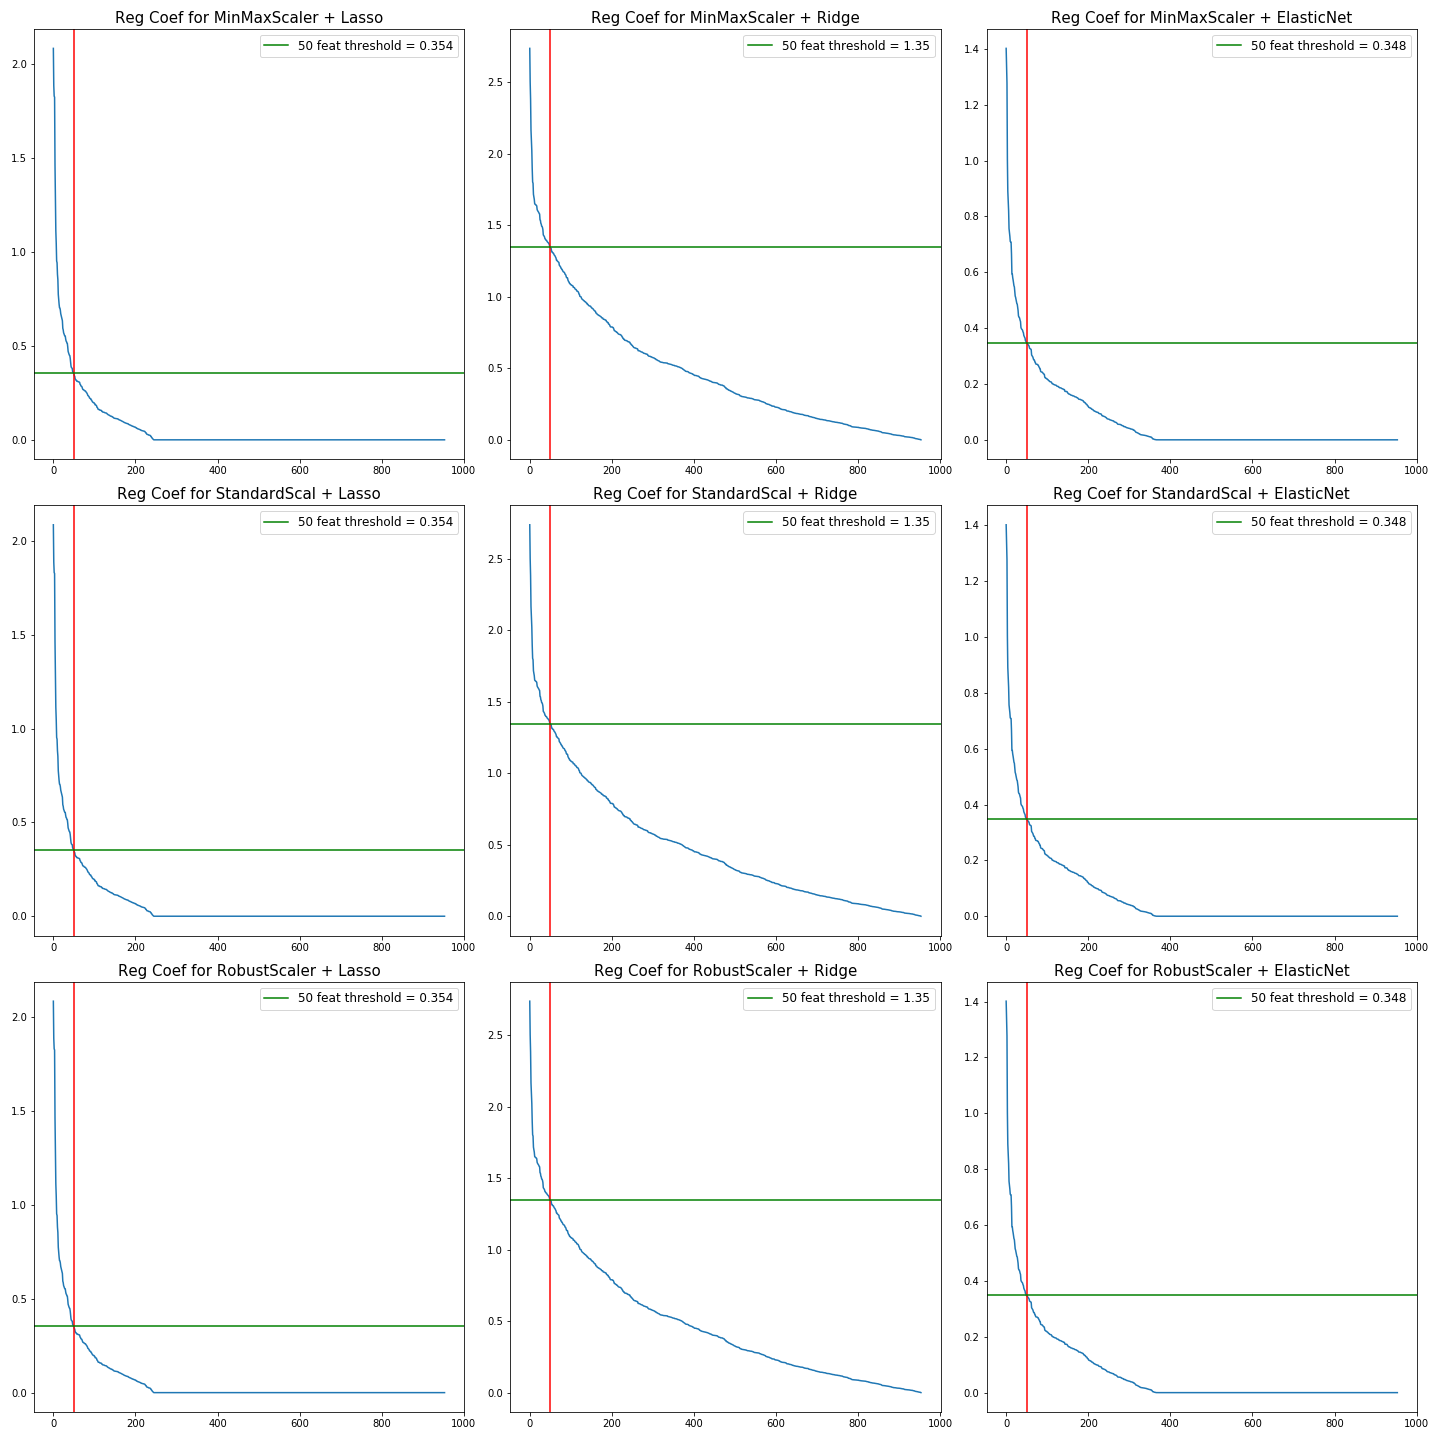
\includegraphics[width=0.7\linewidth]{NineCoefPlot.png}
  \caption{\small{The nine plots that shows the general trend for each one of the scaler + regression combinations. It can be seen that they behave quite the same way. The threshold value does not change at all varying the scaler method, but it depends clearly on the regression method. The vertical red line identify the 50 highest ranked features, while the green horizontal line highlight the threshold value necessary to filter only those features.}}
  \label{fig:NineCoefPlot}
  \end{center}
\end{figure}

What I have actually done was to implement a custom filter for a set of values using the available packages in the library \texttt{scikitlearn}. In this way I was able to perform the succeeding analysis only on a restricted set of features.

\subsection*{Most Influential Features}
The search of the most important features required a ranking system, in order to highlight which ones had generally the highest coefficients among the different regressions. The method I devised it's not based on the effective values of the coefficients but it looks at the 



\subsection*{Regression}
The regression analysis was carried out using a \texttt{GaussianProcessRegressor} performed onto different threshold values on each one of the combinations above and, only at the end, also a single vector regressor (\texttt{SVR}) on the set of features selected.
After any dimensionality reduction one expects a drop in the predictive power of the model, and this was the case. The more I filtered the features, selecting only the most influential, the more the $R^{2}$ score dropped. It was necessary to think up a way to find the best compromise between the $R^{2}$ score and the number of features. Thus I looked for the ratio between these two quantities, in order to select the number at which that value would be the greatest. What I found, as it could be seen in figure 2????? was that also this ratio was dropping as the number of feature was decreasing. Then I chose to use the 50 features with the highest coefficient for the following fine tuning of the parameters. The gaussian process regression in fact do not work well with a too high number of dimension and 50 was chosen as maximum value.


[Figure 2: Ratio plots??]


Before the analysis I split the dataset into two parts: 90\% for the training and the remaining 10\% for the testing part. Then I used the \texttt{GridScearchCV} item from the \texttt{scikitlearn} library to run the complete pipeline described and find out which would be the highest score combination. [Should I report the complete code? pipeline and parameter grid?]. The best result around $0.72$ was given by a single vector regressor, and after a further fine tuning of the parameters the result is $R^{2} = running$. I report the exact set of parametersused to find this results:

bla bla bla bla.

\subsection*{Prediction}
As last step in this data analysis I've used the best regressor to make prediction of age on the test dataset.
Precisely I scaled and filtered according to the most performing combination [find out which is] the test dataset, then used the regressor that was previously fitted on the training dataset as a predictor. What I obtained was a set of predicted ages to be put in relation with the known values of the test data set.
I've decided to use a gaussian process to fit those two set of values, because it is able to provide a good representation of the confidence interval of the prediction over all the range of age.





\end{document}
